% 覆叠空间

%暂时完成,不确定还有什么相关内容值得讲.
\pentry{连续映射和同胚\upref{Topo1}}

覆叠空间是一种常见的简化空间描述的方式,可以更轻松地描述许多复杂空间的性质.覆叠的思想在微分几何中极为重要,而在理论物理中也偶尔会使用该方法.

\subsection{覆叠的概念}
\begin{definition}{覆叠映射和覆叠空间}\label{CovTop_def1}
设有拓扑空间之间的\textbf{满}连续映射$p:C\rightarrow X$.如果对于任意的$x\in X$,存在开集$U_x\in\mathcal{T}_X$且$x\in U_x$,使得$p^{-1}(U_x)$是$C$中若干不相交开子集的并,并且每个这样的开子集都通过$p$和$U_x$同胚,那么称$C$是$X$的\textbf{覆叠空间(covering space)},$p$是其\textbf{覆叠映射(covering map)}或\textbf{覆叠投影(covering projection)}开集$U_x$是点$x$的\textbf{典范邻域}.
\end{definition} 

覆叠映射$p$的逆把典范邻域$U_x$映射为若干个和$U_x$同胚的开集,这也可以表示为存在一个\textbf{离散空间}$F_x$使得$p^{-1}(U_x)\approx U_x\times F_x$.

需要注意的是,覆叠空间并不保证任何邻域都是典范邻域,即不是任何开集$U$的逆映射$p^{-1}(U)$都同构于$U\times F$.

如果$X$是一个连通空间的话,我们还可以得知对于任何典范邻域$U_x$对应的离散空间$F_x$,其基数$\abs{F_x}$都是一样的.这由以下定理严格描述:

\begin{theorem}{连通空间的覆叠}\label{CovTop_the1}
设$p:C\rightarrow X$是一个覆叠映射,$X$是连通的.对于任意的$x, y\in X$,如果记它们的典范邻域分别是$U_x$和$U_y$,且$p^{-1}(U_x)\approx U_x\times F_x$和$p^{-1}(U_y)\approx U_y\times F_y$,则有$\abs{F_x}=\abs{F_y}$.
\end{theorem}
%此定理证明思路较机械,虽简单却步骤繁多,笔者决定暂时略去不讲.

\autoref{CovTop_the1} 意味着如果$X$连通,那么其覆叠映射把它同构到$\abs{F_x}$个自身的拷贝上去了,其中$F_x$是任意点$x\in X$的典范邻域对应的离散空间.

\subsection{覆叠映射的例子}

\begin{example}{}
取实度量空间$\mathbb{R}$和复平面上的单位圆$S^1=\{e^{2\pi\I t}\in\mathbb{C}|t\in\mathbb{R}\}$.建立映射$p:\mathbb{R}\rightarrow S^1$,其中$p(t)=e^{2\pi\I t}$,则$p$是一个覆叠映射,$\mathbb{R}$是$S^1$的覆叠空间.

\begin{figure}[ht]
\centering
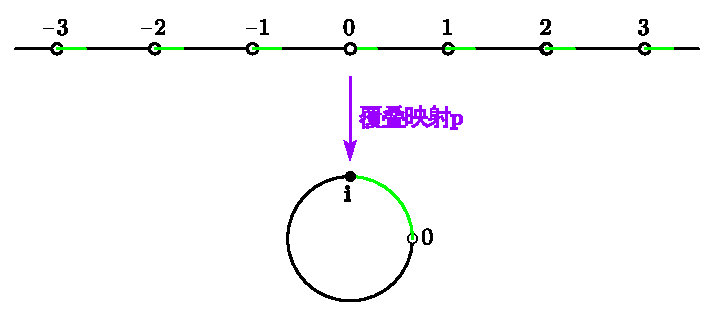
\includegraphics[width=8cm]{./figures/CovTop_1.pdf}
\caption{$\mathbb{R}$到$S^1$的覆叠映射示意图.绿色段分别表示$S^1$上的一个典范邻域和它关于覆叠映射$p$的原像.} \label{CovTop_fig1}
\end{figure}

\end{example}


